\documentclass{article}
\usepackage[utf8]{inputenc}
\usepackage{physics}
\usepackage{amsmath,amssymb}
\usepackage{mathtools}
\usepackage{hyperref}
\usepackage[skip=10pt plus1pt, indent=10pt]{parskip}
\usepackage{float}
\usepackage{pdfpages}
\usepackage{listings}
\usepackage{xcolor}

\definecolor{codegreen}{rgb}{0,0.6,0}
\definecolor{codegray}{rgb}{0.5,0.5,0.5}
\definecolor{codepurple}{rgb}{0.58,0,0.82}
\definecolor{backcolour}{rgb}{0.95,0.95,0.92}

\lstdefinestyle{mystyle}{
    backgroundcolor=\color{backcolour},   
    commentstyle=\color{codegreen},
    keywordstyle=\color{magenta},
    numberstyle=\tiny\color{codegray},
    stringstyle=\color{codepurple},
    basicstyle=\ttfamily\footnotesize,
    breakatwhitespace=false,         
    breaklines=true,                 
    captionpos=b,                    
    keepspaces=true,                 
    numbers=left,                    
    numbersep=5pt,                  
    showspaces=false,                
    showstringspaces=false,
    showtabs=false,                  
    tabsize=2
}

\lstset{style=mystyle}


\DeclareMathOperator{\spn}{span}
\newcommand{\unit}{1\!\!1}

\title{Building the tree}
\date{}

\begin{document}
\maketitle
\begin{abstract}
    We present the precise mathematical algorithm that allows us to calculate how the complexity of a loop circuit grows when adding a specific vertex to a tree-shaped graph state. We then proceed to discuss how this complexity function grows when building the tree in a generic DFS order. We thus show that an optimal DFS order can be found. Furthermore we present a series of elementary bounds for the complexity of the circuit that apply for evey DFS order.
\end{abstract}

\tableofcontents

\newpage
\section{Preliminaries: characterizing the circuit}
Let's start by some definitions.

\textbf{Tree.} A tree is a graph with no cycles. We will use a stronger definition: a tree is a graph with no cycles equipped with a special vertex called $head$ of the the tree. Notice that the presence of the head induces a hierararchy: if we start building the tree from the head, when we add the vertex $v$, we know where to fuse it (to its parent $p(v)$).

\textbf{Order on a tree.} We define an order $O$ on a tree $T$ an array of vertices $[h, v_1, v_2, \dots]$ where $h$ is the head of the tree. This list represents the order in which we want to add the vertices to the tree: thus the parent $p(v)$ of a vertex $v$ must be present in the list before $v$.

\textbf{Depth of a photonic line.} Given a photonic line, there will be a last optical element on this line (remember that in our setup every optical element is a $SU(2)$ matrix that occupies two photonic lines). This optical element will belong to a specific outer loop numbered $n$, we define the \textit{depth} of the photonic line as this number $n$.

\textbf{Complexity of a circuit.} The \textit{complexity} of a circuit is the maximal depth of its photonic lines.

This series of definitions allow us to introduce our main character, the \textit{complexity function} $C(T, O)$:

\textbf{The complexity function.} Given a tree and an order on this tree, this function $C(T, O)$ tells us the number of outer loops needed to implement the circuit.

\newpage

\section{The general algorithm}
\subsection{On the circuit}
We now present a general algorithm to add a new vertex $q_j$ and the edge connecting it to its parent $p(q_j) = q_i$. We need two fundamental blocks:

\textbf{Sinking.}
Sinking a qubit $q$ brings it at the end of the circuit.
\begin{figure}[H]
    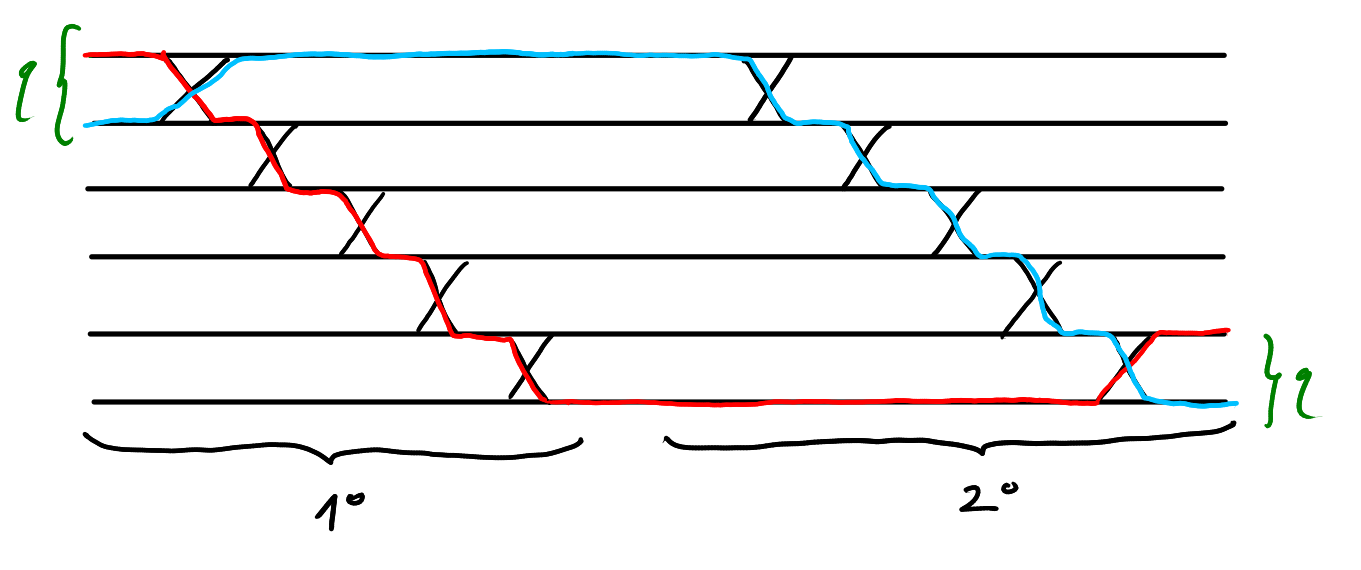
\includegraphics[width=\textwidth]{pics/sinking.png}
\end{figure}

\textbf{Fusing two neighbors qubits.}
\begin{figure}[H]
    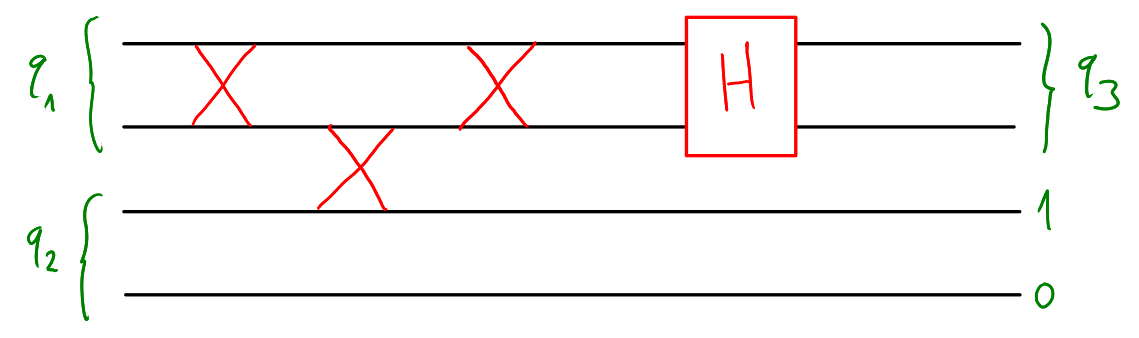
\includegraphics[width=\textwidth]{pics/fusion.png}
\end{figure}

\textbf{The general algorithm.} To add a new vertex $q_j$ and the edge connecting $q_i$ and $q_j$:
\begin{itemize}
    \item we sink $q_i$ at the end of the circuit;
    \item we append a Bell pair at the end of the circuit (made of two qubits $(B_1, B_2)$)
    \item we fuse the now neighbors $q_i$ and $B_1$.
\end{itemize}
\begin{figure}[H]
    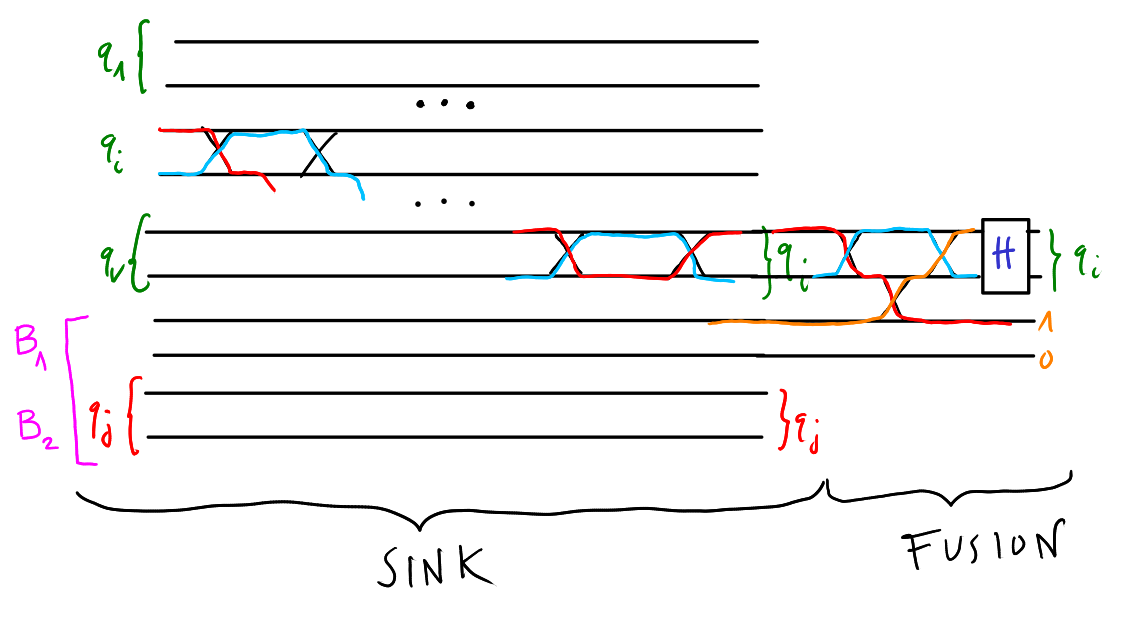
\includegraphics[width=\textwidth]{pics/general_algorithm.png}
\end{figure}


\subsection{On paper}
To get a feeling of what's happening here and how the complexity function grow when adding an edge, let's describe an algorithm to compute $C(T, O)$ for a generic order $O$. Let's start from a crucial observation that will simplify a lot our line of reasoning.

\textbf{Observation.} Every qubit is made of two photonic lines. In general the depth of these two photonic lines may be different. But if we just perform sinking and fusing operations, given a qubit $q$ the two photonic lines that make up the qubit have always the same depth. This allow to define the $depth$ of qubits and not just of photonic lines, given the fact that its photonic lines  have the same depth. Just look at the previous pictures to convince yourself!

We make use of two lists:
\begin{itemize}
    \item \textit{order}: it's an ordered list that follows the order of the qubits in the photonic circuit. Clearly sinking the qubit $q$ places $q$ at the end of $order$. Fusing a at the end of the circuit appends a $1$ to the list order.
    \item \textit{depth}: the element $depth[i]$ gives us the depth of the qubit $order[i]$.
\end{itemize}

Now let's reason on how the two operations of \textit{fusing} and \textit{sinking} act on the two lists:
\begin{enumerate}
    \item \textit{fusing} a qubit $q$ increments $+1$ the last element of $depth$ and then appends a $1$ to the list $depth$; it also appends the value $q$ to the list $order$;
    \item \textit{sinking} a qubit $q$ moves the value $q$ at the end of the list $order$. The action on the depth list is much more complicate. There are two different possible cases:
    \begin{figure}[H]
        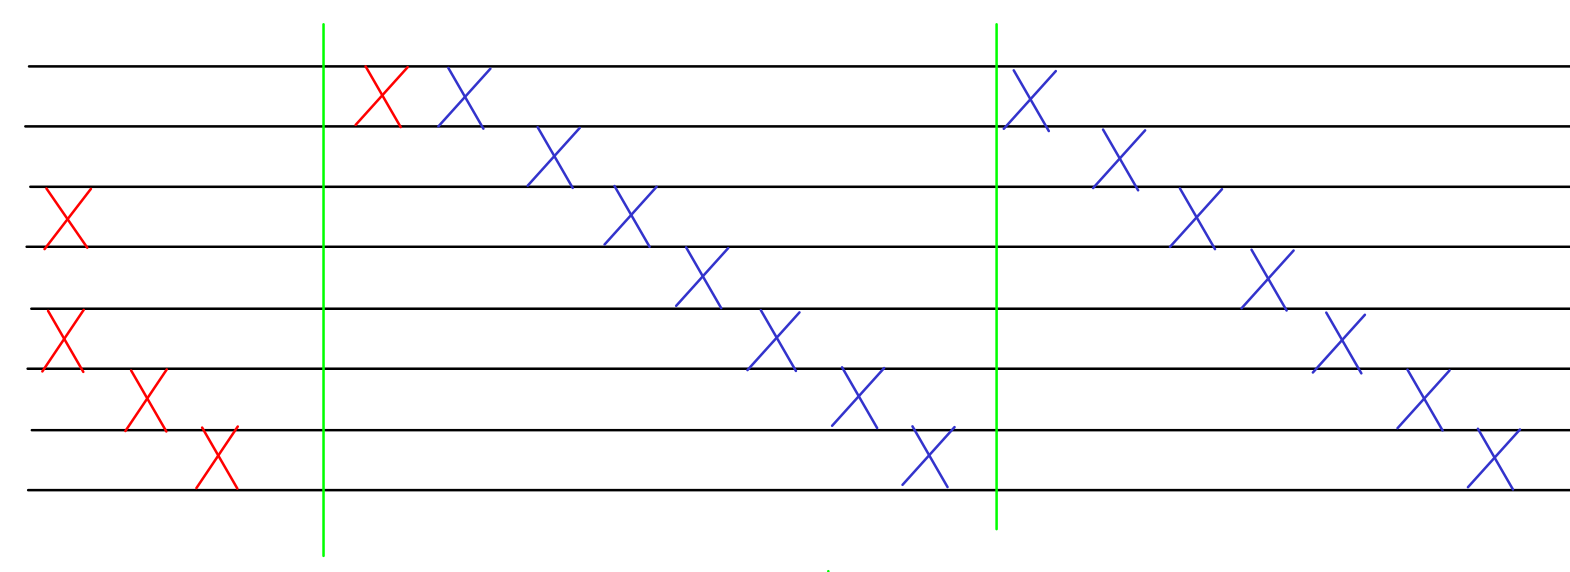
\includegraphics[width=\textwidth]{pics/case_1.png}
        \caption{In the first case the qubit $q$ I want to sink has the biggest depth. In this case I just need one more outer loop.}
    \end{figure}
    \begin{figure}[H]
        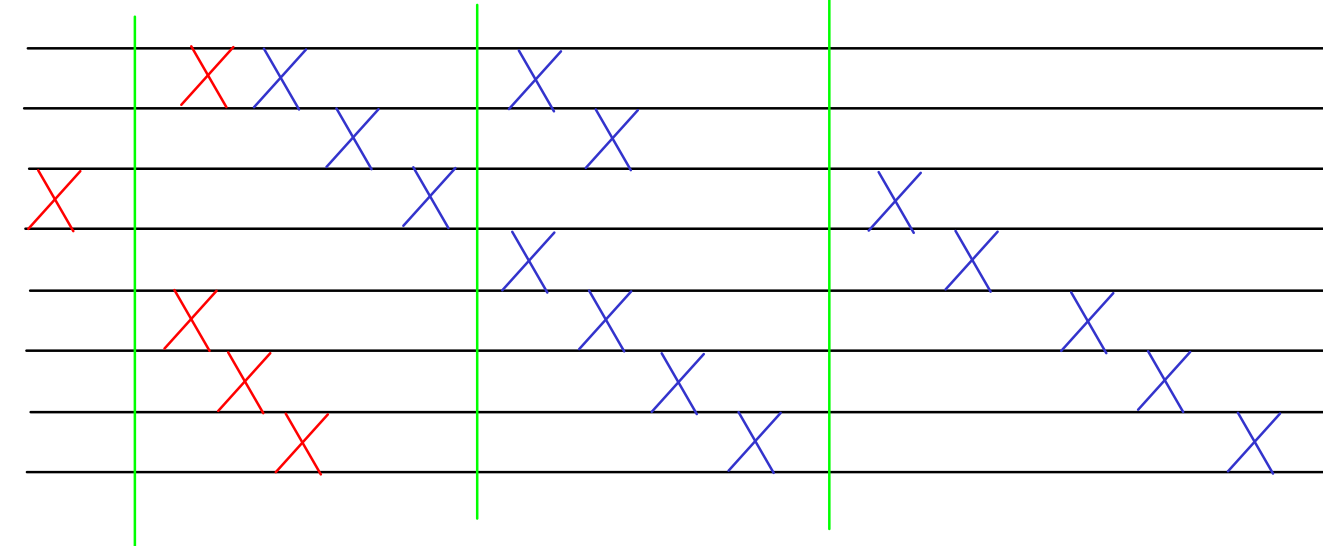
\includegraphics[width=\textwidth]{pics/case_2.png}
        \caption{In the first case the qubit $q$ I want to sink has not the biggest depth (for example there are other qubits with the same depth). In this case I will need two more outer loop.}
    \end{figure}
    
\end{enumerate}

This is summarized in the following function:
\begin{lstlisting}[language=Python]
    #sinking...
    if order.index(parent) < len(order)-1: #check if the parent qubit isn't already at the end of the circuit
            m = depth[order.index(parent)]
            for i in range(order.index(parent)+1, len(order)):
                m = max(m, depth[i]+1)
                depth[i-1] = m+1
                order[i-1] = order[i]
            order[len(order)-1] = parent
            depth[len(order)-1] = m+1

	#fusion...
        depth[len(order)-1] += 1
        order.append(leaf)
        depth.append(1)
\end{lstlisting}

\newpage

\section{Some bounds for the DFS-orders}
\subsection{The main idea}
\begin{figure}[H]
    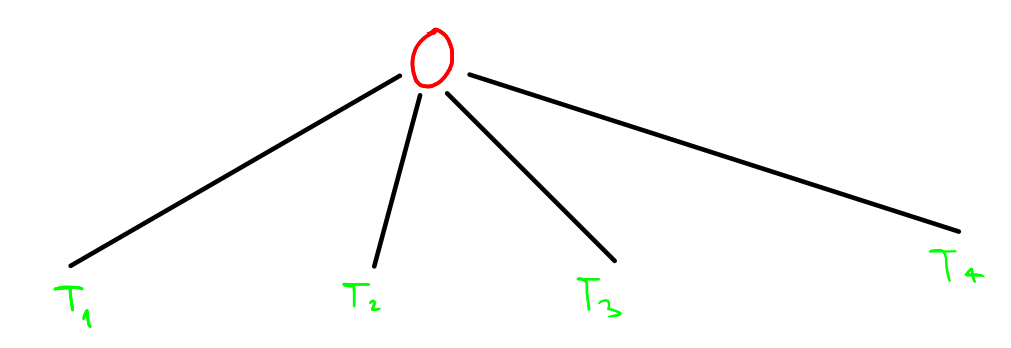
\includegraphics[width=\textwidth]{pics/building_scheme.png}
\end{figure}
Suppose we are building a tree following this scheme and using a DFS-order. The number of outer loops will have the following upper bound:
\begin{align}
    C(T) \leq C(T_1)
\end{align}
after building and attaching the first subtree.
Suppose we attach the second subtree $T_2$:
\begin{align}
    C(T) \leq \max{(C(T_1)+3, C(T_2))}
\end{align}
this is because sinking the $0$ vertex to the bottom of the circuit we use at maximum $C(T_1)+3$ outer loops. And so on:
\begin{align}
    C(T) \leq \max{(\max{(C(T_1)+3, C(T_2))}+3, C(T_3))}\\
    C(T) \leq \max{(\max{(\max{(C(T_1)+3, C(T_2))}+3, C(T_3))}+3, C(T_4))}
    \dots
\end{align}
The expression can be rewritten as:
\begin{align}
    C(T) \leq \max{(C(T_1)+3\times 4, C(T_2)+3\times 3, C(T_3)+3\times 2, C(T_4)+3\times 1, C(T_5))}
\end{align}
This last expression is extremely important and gives us the euristic for the optimal-DFS. To minimize this $\max$ function we want $C(T_1) \leq C(T_2) \leq C(T_3) \dots $. The smallest subtree to the the left! This also explain how to build the worst-DFS.

Similarly we can build a lower bound for $C(T)$, using the fact that:
\begin{align}
    C(T) &\geq \max{(C(T_1)+2, C(T_2))}\\
    &\dots\\
    C(T) &\geq \max{(C(T_1)+2\times 4, C(T_2)+2\times 3, C(T_3)+2\times 2, C(T_4)+2\times 1, C(T_5))}
\end{align}

\subsection{Recursive bounds}
We now present a recursive upper bound that will gift us two nice analytical bounds.

Start by assigning $B(l) = 3$ for every leaf $l$. Now we want to compute the value for some vertex $v$ with children $c_1, c_2, c_n$ ordered by left to right. We have already discussed that:
\begin{align*}
    C(T) &\leq \max(C(c_1)+3\times(n-1), C(c_2)+3\times(n-2),\dots, C(c_n))\\
    &\leq \max(B(c_1)+3\times(n-1), B(c_2)+3\times(n-2),\dots, B(c_n)) \equiv B(v)\\
    &\leq \max(C(c_1), \dots, C(c_n)) + 3\times(n-1)
\end{align*}
The last line tells us how to compute $B(v)$ recursively. Similarly one can construct a lower bound $b(l)$ assigning $b(l)=0$ for every leaf and with the recursive formula:
\begin{align*}
    b(v) \equiv \max(b(c_1)+2\times(n-1), b(c_2)+2\times(n-2),\dots, b(c_n))
\end{align*}

\subsection{Analytical bounds}
\begin{figure}[H]
    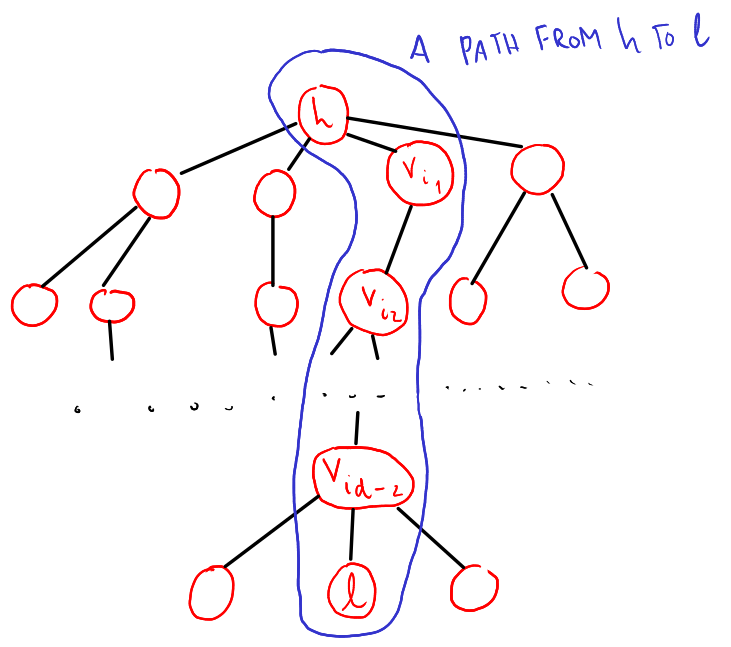
\includegraphics[width=\textwidth]{pics/path.png}
\end{figure}
To find an analytical bounds suppose we have computed the values of $B(v)$ for every vertex recursively. Now, when computing $B(h)$ where $h$ is the head of the tree there will be a children of the head $c(h)_{i_1}$ with $i_1=1, \dots n(h)$ that will have given us the maximum value in the recursive formula:
\begin{align}
    B(h) = B(c(h)_{i_1}) + 3\times(n(h=v_{i_0})-i_1)
\end{align}
where $n(h)$ is the number of children of the head vertex and $d$ is the depth of the tree. So we can construct this sequence of vertices $$v_{i_0} = h, c(h)_{i_1}, v_{i_2}, \dots, v_{i_{d-2}},v_{i_{d-1}}=l$$ going from the head to a leaf where $l$. Here $i_1, i_2, \dots$ represent the positioning of the vertex in the children list. Clearly vertex $v_{i_k}$ is a children of $v_{i_{k-1}}$ and $i_k = 1, \dots, n(v_{i_{k-1}}$).
The upper bound for the head will thus be:
\begin{align*}
    B(h) &= 3 + 3\times(n(v_{i_{d-2}})-i_{d-1})+\dots+3\times(n(v_{i_0})-i_1)\\
    &\leq 3+3\left[(n(v_{i_{d-2}})-1)+\dots+(n(v_{i_{0}})-1)\right]\\
    &= 3+3\left[n(v_{i_{d-2}})+\dots+n(v_{i_{0}})-(d-1)\right]
\end{align*}
In particular, given a path starting from the head and going to a leaf:
$$p_0 = h, p_1, \dots, p_{d-2}, p_{d-1} = l$$ we have
\begin{align}
    B(h) &\leq 3+\max_{\text{all paths}}[n(p_{d-2})+\dots+n(p_{0})-(d-1)]\\
    &\leq 3 + (N-1)(d-1)
\end{align}
where $N$ is the maximum of $n(v)$ over all vertices in the tree.

One could also think if it's possible to build an analytical lower bound. Using $i_k \leq n(v_{i_{k-1}})$ one would trivially get $b(h) \geq 0$. This makes sense because a linear cluster takes only has $C(T) = 2$.

A trivial upper bound valid for every order $O$ is $C(T) \leq 3V$.

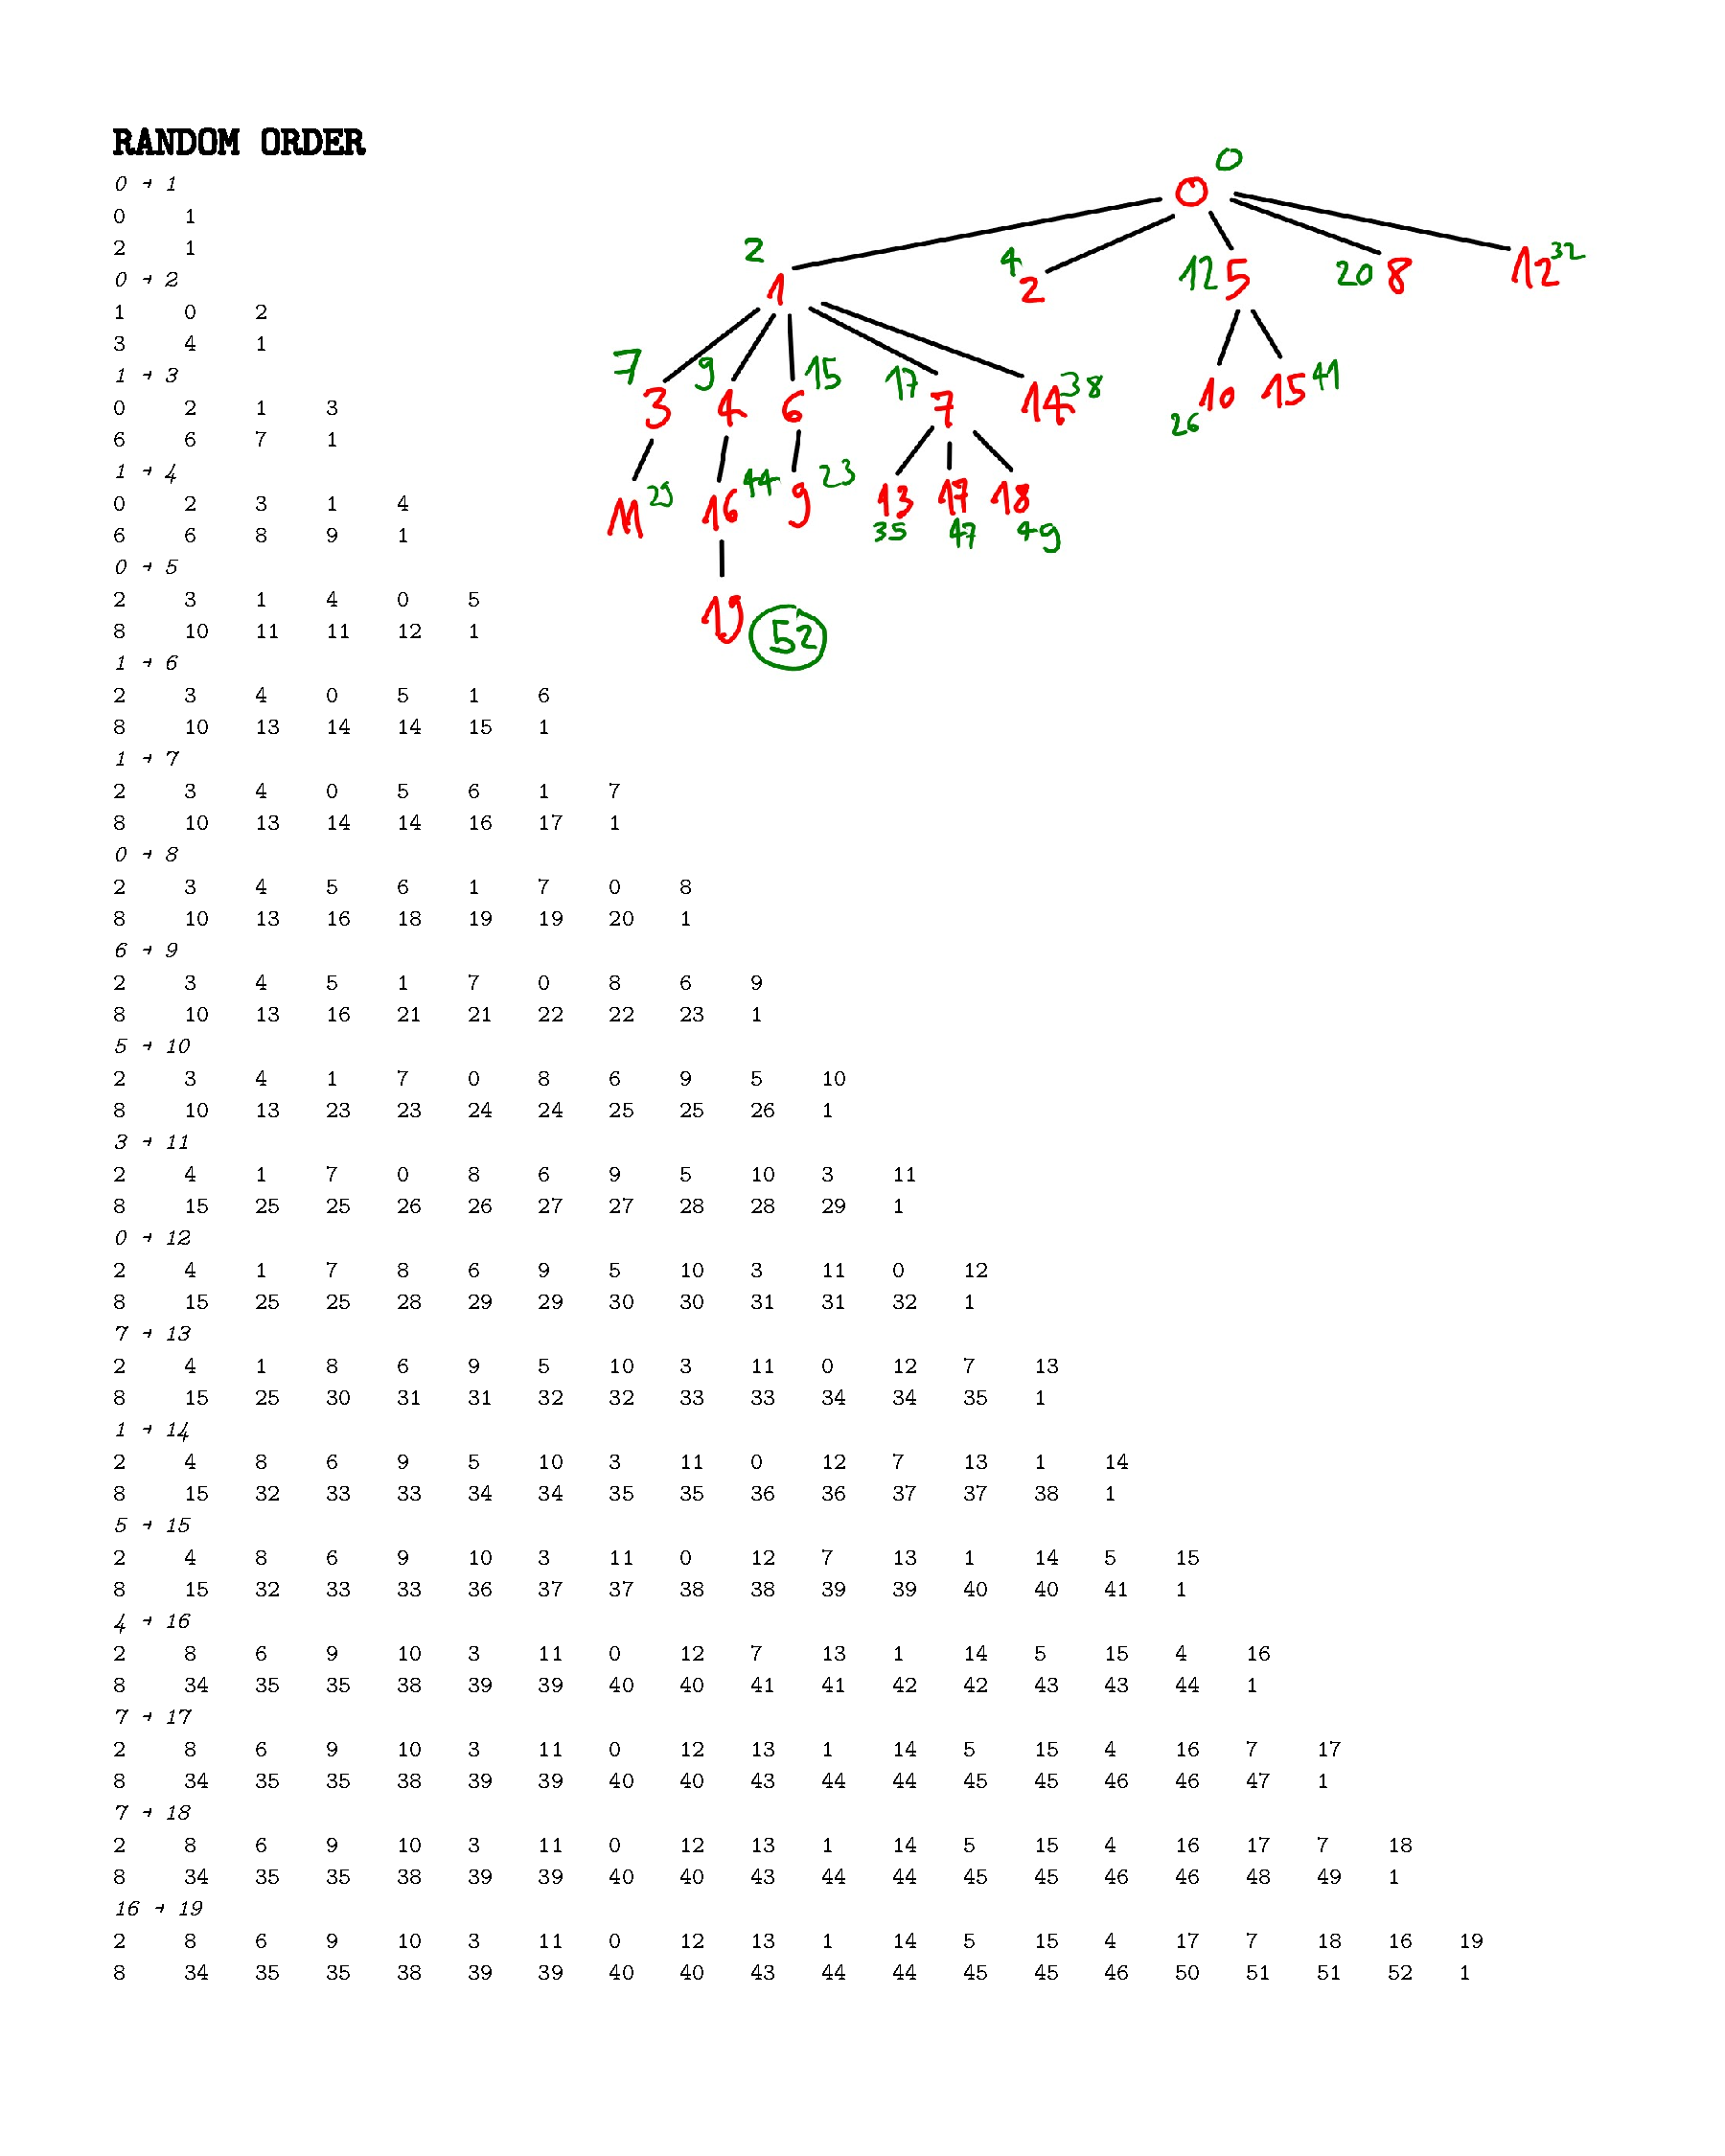
\includepdf[pages={-}]{analysis_drawed.pdf}

\end{document}